\documentclass[convert={outext=.svg,command=\unexpanded{pdf2svg \infile\space\outfile}},multi=false]{standalone}

\usepackage{auto-pst-pdf}
\usepackage{pst-optic}

\usepackage{arev}
\usepackage[T1]{fontenc}
\usepackage{soul}

\begin{document}

%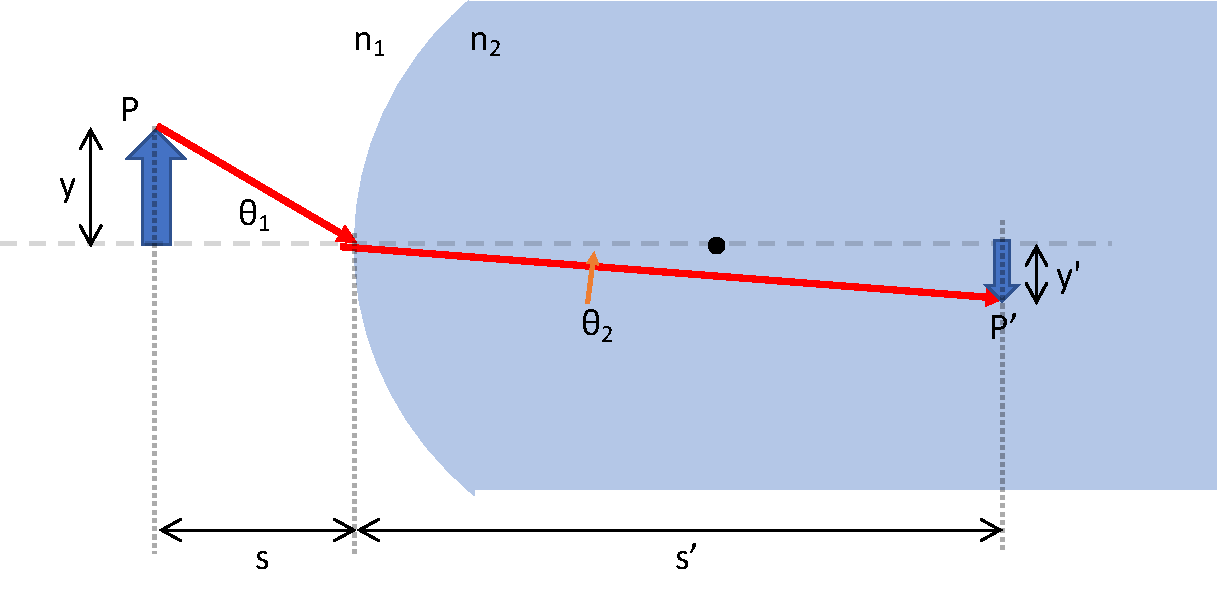
\includegraphics[scale=0.7]{ch16-sphsurfacemag}

\begin{pspicture}[showgrid=false]%(-10cm,-10cm)(10cm,10cm) 


\rput(0,0){
\lens[
lensType = CVG,
lensGlass=true,
lensHeight=3.5cm,
%linewidth=0.2mm,
%linestyle=dashed,
lensWidth=0.25,
drawing=false]
}

\rput(3,0){
\lens[
lensType = CVG,
lensHeight=3.5cm,
lensGlass=true,
alpha=0.5,
linestyle=dotted,
lensWidth=0.15,
drawing=false]
}

\rput(0,0){%
\newpsstyle{opticalAxis}{linewidth=0.5pt,linecolor=gray,linestyle=dashed}
\lens[
lensType=CVG,
lensGlass,
lensHeight=3.5cm,
lensWidth=0.25,
rayColor=red, 
linestyle=dashed,
%linewidth=0.2mm,
focus=2.25,
AB=1,
OA=-4.25,
spotO=270,
spotAi=90,
spotBi=270,
spotFi=100,
nameFi=F_1',
nameF=F_1,
]}

\psline[linecolor=red]{}(0,1)(3,-0.335)
\psline[linecolor=red]{}(-4.25,1)(3,-0.705)
\psline[linecolor=red]{}(-4.25,1)(0,-1.125)
\psline[linecolor=red]{}(0,-1.125)(3,-1.125)
\psline[linecolor=red]{}(-4.25,1)(0,1)
\psline[linecolor=black,linewidth=0.5mm]{}(-4.25,1)(-4.25,0)
%\psline[linecolor=gray]{}(-10,0)(16,0)



%\psdot*(0,0)
%\psline{|<->|,gray}(0,-2)(-7,-2)
%\uput[d](-3.5,-2){$s$}
%\psline{|<->|,gray}(0,-2)(3.95,-2)
%\uput[d](1.75,-2){$s'$}

%\psline{|<->|,gray}(-7.5,0)(-7.5,2)
%\uput[l](-7.5,1){$y$}
%\psline{|<->|,gray}(4.2,0)(4.2,-1.1)
%\uput[r](4.2,-0.5){$y'$}

%\uput[](-1.75,0.25){$\theta$}
%\uput[](1.75,-0.25){$\theta$}
%\ncline{<->}{lens}{object}
%\uput[d](-3,0){F}
\end{pspicture}

\end{document}